%%% D\'ebut du pr\'eambule %%%

%%%%%%%%%%%%%%%%%%%%%%%%%%%%%%%%%
% Options g\'en\'erales du document %
%%%%%%%%%%%%%%%%%%%%%%%%%%%%%%%%%

\documentclass[12pt]{report}	% Classe du document

%%%%%%%%%%%
% Langues %
%%%%%%%%%%%

\usepackage[english]{babel}		% Francisation de LaTeX

%%%%%%%%%%%%%%%%%%%%%%%
% Encodage, fontes... %
%%%%%%%%%%%%%%%%%%%%%%%


\usepackage[T1]{fontenc}
\usepackage[latin9]{inputenc}
\usepackage{amssymb}

\usepackage{latexsym}
\usepackage{amsmath}
%\usepackage{graphicx}
\usepackage{aeguill}
\usepackage{aecompl}
\usepackage{url}
\usepackage{scribe_MG}
 		% Encodage d'entr\'ee : permet l'utilisation de caract\`eres accentu\'es en entr\'ee


\usepackage{graphicx}			% pour les images

%%% Fin du pr\'eambule %%%
\def\ts{\top}
\def\XX{\mathbf{X}}
\def\wb{\mathbf{w}}
\def\xb{\mathbf{x}}
\def\yb{\mathbf{y}}
\def\db{\mathbf{d}}
\def\hb{\mathbf{h}}
\def\Diag{\text{Diag}}

\def\etab{\boldsymbol \eta}

%%% D\'ebut du document %%%

\begin{document}
	 
\scribe{Aymeric Reshef, Claire Vernade}
\lecturenumber{2}			% required, must be a number
\lecturedate{October 11}		% required, omit year

	
\maketitle

%	\underline{For your information}\\
\BIT
\item
Course webpage: 
\url{http://www.di.ens.fr/~fbach/courses/fall2013/}
\EIT

\section{Single node models (last part)}


The previous course introduced the notion of \emph{Maximum Likelihood Estimator} (MLE). Basic examples on Bernoulli model, multinomial model and Gaussian model were explicited, and side notes detailed the use of Lagrangian operators and of differentials. The last example was using the multivariate Gaussian model. We recall it briefly in the next subsection.

\subsection{The Multivariate Gaussian model}

If $X$ is a random variable taking values in $\mathbb{R}^{d}$. Let $\mu\in\mathbb{R}^{d}$ and $\Sigma\in\mathbb{R}^{d\times d}$ be a positive definite matrix. $X$ follows a \emph{multivariate Gaussian model} (denoted by $X\sim\mathcal{N}\left(\mu,\Sigma\right)$) if
\[
p_{\mu,\Sigma}\left(\xb\right)=\frac{1}{\sqrt{\left(2\pi\right)^{d}\det\Sigma}}\exp\left(-\frac{1}{2}\left(\xb-\mu\right)^{\ts}\Sigma^{-1}\left(\xb-\mu\right)\right).
\]

Let $X_{1},\cdots,X_{n}\sim\mathcal{N}\left(\mu,\Sigma\right)$, $iid$. Then, the negative \emph{log-likelihood} of the joint distribution is
\begin{eqnarray*}
-l\left(\mu,\Sigma\right) & = & -\sum_{i=1}^{n}\log p_{\mu,\Sigma}\left(\xb_{i}\right)\\
 & = & \frac{nd}{2}\log\left(2\pi\right)+\frac{n}{2}\log\left(\det\Sigma\right)+\frac{1}{2}\sum_{i=1}^{n}\left(\xb_{i}-\mu\right)^{\ts}\Sigma^{-1}\left(\xb_{i}-\mu\right).
 \end{eqnarray*}

Its gradient with respect to $\mu$ is given by
\begin{eqnarray*}
-\nabla_{\mu}l\left(\mu,\Sigma\right) & = & \sum_{i=1}^{n}\Sigma^{-1}\left(\xb_{i}-\mu\right)\\
 & = & \Sigma^{-1}\left(\sum_{i=1}^{n}x_{i}-n\mu\right) = \Sigma^{-1}\left(n\bar{x}-n\mu\right),
 \end{eqnarray*}
 which leads to \fbox{$\hat{\mu} = \frac{1}{n}\bar{x}$}\,, the empirical mean.
 
 In order to compute the gradient with respect to $\Sigma$, we first write $A=\Sigma^{-1}$, so that
\begin{eqnarray*}
-l\left(\mu,\Sigma\right) & = & \frac{nd}{2}\log\left(2\pi\right)-\frac{n}{2}\log\left(\det A\right)+\frac{1}{2}\sum_{i=1}^{n}\left(\xb_{i}-\mu\right)^{\ts}A\left(\xb_{i}-\mu\right)\\
&=&\frac{nd}{2}\log\left(2\pi\right)-\frac{n}{2}\log\left(\det A\right)+\frac{n}{2}\tr(A\tilde{\Sigma}),
 \end{eqnarray*}
where we introduced the empirical covariance matrix $\tilde{\Sigma}$ defined as
\[
\tilde{\Sigma} = \frac{1}{n}\sum_{i=1}^n\left(\xb_{i}-\mu\right)^{\ts}\left(\xb_{i}-\mu\right).
 \]
 The matrix $A$ appears in the expression of the log-likelihood in two terms: $\frac{n}{2}\log\det A$ and $\frac{n}{2}\tr(A\tilde{\Sigma})$.\\
 Denote by $f(A) = \tr(A\tilde{\Sigma})$. Then
 $f(A+H)-f(A) = \tr(H\tilde{\Sigma})$,
 which leads to $\nabla f (A) = \tilde{\Sigma}$.\\ 
 Now, write $\log\det A$ as
 \[
 \log\det (A+H) =  \log\det \left( A^\frac{1}{2}\left(I+A^{-\frac{1}{2}}HA^{-\frac{1}{2}}\right)A^\frac{1}{2} \right) = \log\det A + \log\det (I+\tilde{H})
 \]
 where $A^\frac{1}{2}$ stands for the square root matrix of $A$ (it exists, since $A$ is positive definite) and $\tilde{H} = A^{-\frac{1}{2}}HA^{-\frac{1}{2}}$. Let's see how $\log\det (I+\tilde{H})$ looks like. Noting that $\log\det I = 0$, and denoting by $(\lambda_1,\cdots ,\lambda_d)$ the eigenvalues of $\tilde{H}$, we have that
 \[
\log\det (I+\tilde{H}) = \log\det (I+\tilde{H})-\log\det I = \sum_{j=1}^d\log(1+\lambda_j) \approx \sum_{j=1}^d\lambda_j + o(\lVert \tilde{H} \rVert).
 \]
 But then,$$\sum_{j=1}^d\lambda_j = \tr(\tilde{H}) = \tr(A^{-\frac{1}{2}}HA^{-\frac{1}{2}}) = \tr(HA^{-1}).$$We conclude that $\nabla_A \log\det A = A^{-1}$.
 
 Plugging these results into the gradient of the log-likelihood with respect to $A$, we have
 \[
 \nabla_A l(A) = -\frac{n}{2}A^{-1}+\frac{n}{2}\tilde{\Sigma}.
 \]
 The optimality condition $\nabla_A l(A)$ leads to $A^{-1} = \tilde{\Sigma}$, which means that\begin{center}\fbox{$\hat{\Sigma} = \frac{1}{n}\sum_{i=1}^n\left(\xb_{i}-\mu\right)^{\ts}\left(\xb_{i}-\mu\right)$}\end{center} is the empirical covariance matrix.
 
 Note that we assumed that $A$ was invertible, which is an implicit condition when writing $\log\det A$. This implies that in a rigorous sense the maximum likelihood estimator is undefined when $\tilde{\Sigma}$ is not invertible. In practice, the MLE is extended by continuity to the rank deficient case.
 
 \section{Models with two nodes}
 
In this section, we work with two nodes: one node corresponds to an input $X$, and one node corresponds to an output $Y$.

Recall that when dealing with two random variables $X$ and $Y$, one can use a \emph{generative} model, i.e.\ which models the joint distribution $p(X,Y)$, or one can use instead a \emph{conditional} model (often considered equivalent to the slightly different concept of \emph{discriminative model}), which models the conditional probability of the output, given the input $p(Y|X)$. The two following models, \emph{linear regression} or a \emph{logistic regression}, are \emph{conditional models}.

\subsection{Linear regression}

Let's assume that $Y\in\mathbb{R}$ depends linearly on $X\in\mathbb{R}^p$. Let $w\in\mathbb{R}^p$ be a weighting vector and $\sigma^2>0$. We make the following assumption:
$$Y \mid X \sim \mathcal{N}({\wb}^{\ts}   X,\sigma^2),$$
which can be rewritten as
$$Y = {\wb}^{\ts}X+\epsilon,$$
with $\epsilon \sim \mathcal{N}(0,\sigma^2)$. Note that if there is an offset $w_0\in\mathbb{R}^p$, that is, if $Y = {\wb}^{\ts}X+w_0+\epsilon$, one can always redefine a weighting vector $\tilde{\wb}\in\mathbb{R}^{p+1}$ such that $$Y=\tilde{\wb}^{\ts}\begin{pmatrix}x\\1\end{pmatrix}+\epsilon.$$

Let $\mathcal{D}=\lbrace (\xb_1,y_1),\cdots ,(\xb_n,y_n)\rbrace$ be a training set of i.i.d.\ random variables. Each $y_i$ is a \emph{label} (a decision) on observation $\xb_i$. We consider the \emph{conditional} distribution of all outputs given all inputs, which is a product of terms because of the independence of the pairs forming the training set:
$$
p(y_1, \cdots , y_n | x_1, \cdots, x_n ; {\wb},\sigma^2) = \prod_{i=1}^n p(y_i | \xb_i ; {\wb},\sigma^2).
$$
The associated log-likelihood has the following expression:
$$
-l({\wb},\sigma^2) = -\sum_{i=1}^n{\log p(y_i|\xb_i)} = \frac{n}{2}\log(2\pi\sigma^2)+\frac{1}{2}\sum_{i=1}^n{\frac{(y_i-{\wb}^{\ts}\xb_i)^2}{\sigma^2}}.
$$
The minimization problem with respect to $w$ can now be reformulated as:
$$
\begin{array}{ll}
\mathrm{find} & \hat{\wb} = \argmin_{\wb} \frac{1}{2n}\sum_{i=1}^n{(y_i-{\wb}^{\ts}\xb_i)^2}.
\end{array}
$$
Define the so-called \emph{design matrix} $\XX$ as
$$
\XX = \begin{pmatrix}
\xb_1^{\ts} \\ \vdots \\ \xb_n^{\ts}
\end{pmatrix} \in \mathbb{R}^{n\times p}
$$
and denote by $\yb$ the vector of coordinates $(y_1,\cdots ,y_n)$. The minimization problem over $w$ can be rewritten in a more compact way as:
$$
\begin{array}{ll}
\mathrm{find} & \hat{\wb} = \argmin_{\wb} \frac{1}{2n}{\lVert \yb - \XX\wb \rVert}^2.
\end{array}
$$
Let $f:w\mapsto\frac{1}{2n}{\lVert \yb - \XX\wb \rVert}^2 = \frac{1}{2n}(\yb^{\ts}\yb-2{\wb}^{\ts}\XX^{\ts}\yb +{\wb}^{\ts}\XX^{\ts}\XX\wb$. $f$ is strictly convex if and only if its Hessian matrix is invertible. This is never the case when $n<p$ (in this case, we deal with underdetermined problems). Most of the time, the Hessian matrix is invertible when $n \geq p$. When this is not the case, we often use the Tikhonov regularization, which adds a penalization of the $\ell_2$-norm of $w$ by minimizing $f({\wb})+\lambda{\lVert \wb \rVert}^2$ with some hyperparameter $\lambda>0$.

The gradient of $f$ is
$$
\nabla f({\wb}) = \frac{1}{n}\XX^{\ts}(\XX\wb-\yb ) = 0 \iff \XX^{\ts}\XX\wb = \XX^{\ts}\yb .
$$
The equation \fbox{$\XX^{\ts}\XX\wb = \XX^{\ts}\yb $} is known as the \emph{normal equation}. If $\XX^{\ts}\XX$ is invertible, then the optimal weighting vector is
\begin{center}
\fbox{$\hat{\wb} = (\XX^{\ts}\XX)^{-1}\XX^{\ts}\yb  = \XX^\dagger \yb$}
\end{center}
where $\XX^\dagger = (\XX^{\ts}\XX)^{-1}\XX^{\ts}$ is the \emph{Moore-Penrose pseudo-inverse} of $X$. If $\XX^{\ts}\XX$ is not invertible, the solution is not unique anymore, and for any $\hb\in\ker(\XX)$, $\hat{\wb} = (\XX^{\ts}\XX)^\dagger \XX^{\ts}\yb +\hb$ is an admissible solution. In that case however it would be necessary to use regularization.

The computational cost to evaluate the optimal weighting vector from $\XX$ and $\yb$ is $O(p^3)$ (use a Cholesky decomposition of matrix $\XX^{\ts}\XX$ and solve two triangular systems).

Now, let's differentiate $l({\wb},\sigma^2)$ with respect to $\sigma^2$: we have
$$
\nabla_{\sigma^2}l({\wb},\sigma^2) = \frac{n}{2\sigma^2}-\frac{n}{2\sigma^4}\frac{1}{n}\sum_{i=1}^n{(y_i-{\wb}^{\ts}\xb_i)^2}.
$$
Setting $\nabla_{\sigma^2}l({\wb},\sigma^2)$ to zero gives \begin{center}\fbox{$\hat{\sigma}^2 = \frac{1}{n}\sum_{i=1}^n{(y_i-{\wb}^{\ts}\xb_i)^2}$.}
\end{center}

In practice, whenever we use a data matrix $\XX$ in machine learning, we first preprocess it to try and avoid that it would be too badly conditioned, so to avoid numerical issues. Two main operations are applied columnwise: first, a centering (remove the mean of the coefficients) and a normalization (divide coefficients from a column by the standard deviation of the column vector). Note that this preprocessing *does not guarantee* that the matrix we obtain is well-conditioned: in particular, it can be low rank... 

\subsection{Logistic regression}

Let $X\in\mathbb{R}^p$, $Y\in\lbrace 0,1 \rbrace$. We assume that $Y$ follows a Bernoulli distribution with parameter $\theta$. The problem is to find $\theta$. Let's define the \emph{sigmoid} function $\sigma$ defined on the real axis and taking values in $[0,1]$, such that $$\forall z \in \mathbb{R}, \sigma(z) = \frac{1}{1+e^{-z}}.$$The sigmoid function is plot on Figure~\ref{fig:sigmoid}.

\begin{figure}
\begin{center}
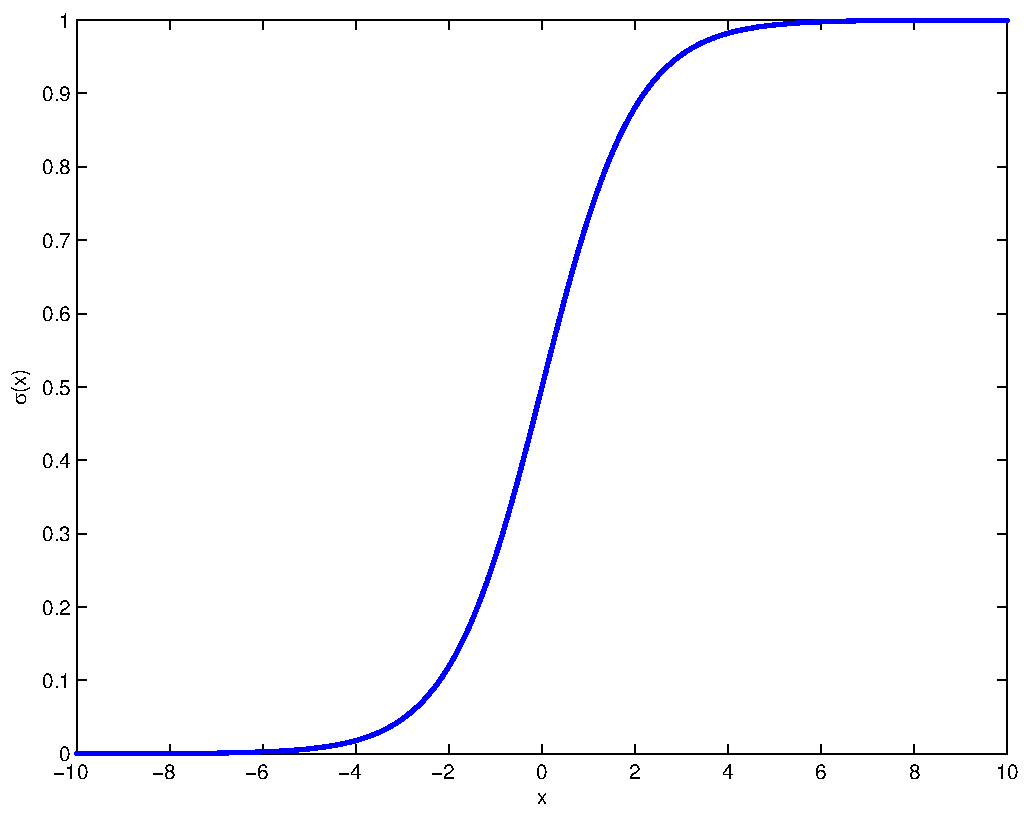
\includegraphics[width=.5\linewidth]{figures/sigmoid-eps-converted-to.pdf}
\caption{\label{fig:sigmoid}Sigmoid function.}
\end{center}
\end{figure}

One can easily prove that
$$
\begin{array}{lll}
\forall z \in \mathbb{R},& \sigma(-z)&=1-\sigma(z),\\
\forall z \in \mathbb{R},& \sigma ' (z) &= \sigma(z)(1-\sigma(z)) = \sigma(z)\sigma(-z).
\end{array}
$$

We now assume that, for a given observation $X=\xb$, the output $Y{|X=\xb}$ follows a Bernoulli law with parameter $\theta=\sigma({\wb}^{\ts}\xb)$, where $w$ is again a weighting vector. In practice, we still can add an offset ${\wb}^{\ts}\xb+w_0$. Then, the conditional distribution is given by
$$
p(Y=y|X=\xb) = \theta^y(1-\theta)^{1-y} = \sigma({\wb}^{\ts}\xb)^y\sigma(-{\wb}^{\ts}\xb)^{1-y}.
$$
Given a training set $\mathcal{D}=\lbrace (\xb_1,y_1),\cdots ,(\xb_n,y_n)\rbrace$ of $iid$ random variables , we can compute the log-likelihood
$$
l({\wb}) = \sum_{i=1}^n{y_i\log\sigma({\wb}^{\ts}\xb_i)+(1-y_i)\log\sigma(-{\wb}^{\ts}\xb_i)}.
$$
In order to minimize the log-likelihood, since $z\mapsto \log(1+e^{-z})$ is a convex function and $\wb\mapsto {\wb}^{\ts}\xb_i$ is linear, we calculate its gradient. We write $\eta_i = \sigma(\theta^{\ts}\xb_i)$:
$$\nabla_{\wb} l({\wb}) = \sum_{i=1}^n y_i\xb_i \frac{\sigma({\wb}^{\ts}\xb_i)\sigma(-{\wb}^{\ts}\xb_i)}{\sigma({\wb}^{\ts}\xb_i)} -(1-y_i)\xb_i\frac{\sigma({\wb}^{\ts}\xb_i)\sigma(-{\wb}^{\ts}\xb_i)}{\sigma(-{\wb}^{\ts}\xb_i)} = \sum_{i=1}^n \xb_i(y_i-\eta_i)$$
Thus, $\nabla_{\wb} l({\wb}) = 0 \iff \sum_{i=1}^n \xb_i(y_i-\sigma(\theta^{\ts}\xb_i))=0$. This equation is nonlinear and we need an iterative optimization method to solve it. For this purpose, we derive the Hessian matrix of $l$:
$$
Hl({\wb}) = \sum_{i=1}^n {\xb_i(0-\sigma '({\wb}^{\ts}\xb_i)\sigma '(-{\wb}^{\ts}\xb_i)\xb_i^{\ts})}\\
$$
$$
= \sum_{i=1}^n{(-\eta_i(1-\eta_i))\xb_i\xb_i^{\ts}} = -\XX^{\ts}\Diag(\eta_i(1-\eta_i))\XX\\
$$

where $\XX$ is the design matrix defined previously.

In the following we discuss first- and second-order optimization methods and apply them to  logistic regression.

\subsubsection{First-order methods}

Let  $f:\mathbb{R}^p \rightarrow \mathbb{R}$ be the convex $C^{1}$ function that we want to minimize. A \emph{descent direction} at point $\xb$ is a vector $d$ such that $\langle \db, \nabla f (\xb) \rangle < 0$. The minimization of $f$ can be done by applying a \emph{descent algorithm}, which iteratively takes a step in a descent direction, leading to an iterative scheme of the form
$$
 \xb^{(k+1)}=\xb^{(k)}+\varepsilon^{(k)} \db^{(k)},
$$
where $\varepsilon^{(k)}$ is the \emph{stepsize}. The direction $\db^{(k)}$ is often chosen as the opposite of the gradient of $f$ at point $\xb^{(k)}$: $\db^{(k)} = -\nabla f (\xb^{(k)})$.

There are several choices for $\varepsilon^{(k)}$:
\begin{enumerate}
\item Constant step: $\varepsilon^{(k)}=\varepsilon$. But the scheme does not necessarily converge.
\item Decreasing step size: $\varepsilon^{(k)}\propto\frac{1}{k}$
with $\sum_{k}{\varepsilon^{(k)}}=\infty$ and $\sum_{k}{(\varepsilon^{(k)})^{2}}<\infty$. The scheme is guaranteed to converge.
\item One can determine $\varepsilon^{(k)}$ by doing a \emph{Line Search} which tries to find $\min_{\varepsilon}f(\xb^{(k)}+\varepsilon \db^{(k)})$: 
\begin{itemize}
\item either exactly but this is costly and rather useless in many situations; 
\item or approximately (see the Armijo linesearch). This is a better method. 
\end{itemize}
\end{enumerate}

\subsubsection{Second-order methods}
This time, let  $f:\mathbb{R}^p \rightarrow \mathbb{R}$ be the  $C^{2}$ function that we want to minimize. We write the second-order Taylor-expansion of $f$:
$$
f(\xb)=f(\xb^t)+(\xb-\xb^t)^{\ts}\nabla f(\xb^t)+\frac{1}{2}(\xb-\xb^t)^{\ts} Hf(\xb^t)(\xb-\xb^t)+o(\left \Vert \xb-\xb^t \right \Vert ^2) \\
\overset{def}{=} g_t(\xb) + (\left \Vert \xb-\xb^t \right \Vert ^2)\\
$$
A local optimum $\xb^*$ is then reached when 
$$\begin{cases}
\nabla f(\xb^{*})=0\\
H(f(\xb^{*})\succeq 0\\
\end{cases}$$

In order to solve such a problem, we are going to use \emph{Newton's method}. If $f$ is a convex function, then $\nabla g_t(\xb) = \nabla f(\xb^t) + Hf(\xb^t)(\xb-\xb^t)$ and we only need to find $\xb^{*}$ so that $\nabla g_t(\xb) =0$, $ie$. we set $\xb^{t+1} = \xb^t - [Hf(\xb^t]^{-1}\nabla f(\xb^t)$. If the Hessian matrix is not invertible, we can regularize the problem and minimize $g_t(\xb)+\lambda {\lVert \xb-\xb^t \rVert}^2$ instead.

In general the previous update, called the \emph{Pure Newton step} does not lead to a convergent algorithm even if the function is convex!

In general it is necessary to use the so-called \emph{Damped Newton method}, to obtain a convergent algorithm which consists in doing the following iterations:
$$
 \xb^{t+1}=\xb^{t}-\varepsilon^{t}(Hf(\xb^t))^{-1}\nabla f (\xb^t), 
$$
where $\varepsilon ^t$ is set with the Armijo \emph{Line Search}

This method may be computationally costly in high dimension because of the inverse of the hessian matrix that needs to be computed at each iteration. For some functions, however, the pure Newton's method does converge. This is the case for logistic regression.

In the context of non-convex optimization, the situation is more complicated because the Hessian can have negative eigenvalues. In that case, so-called trust region methods are typically used.

\subsubsection{Application to logistic regression}

We will write the form that Newton's algorithm takes for logistic regression. We had :
\begin{eqnarray*}
l({\wb}) &=& \sum_{i=1}^n{y_i\log\sigma({\wb}^{\ts}\xb_i)+(1-y_i)\log\sigma(-{\wb}^{\ts}\xb_i)}\\
\nabla _{\wb}l({\wb}) &=& \sum_{i=1}^n \xb_i(y_i-\eta_i) = \XX^{\ts}(\yb-\etab)\\
Hl({\wb}) &=& -\XX^{\ts}\Diag(\eta_i(1-\eta_i))\XX\\
\end{eqnarray*}
The second-order Taylor expansion of the loss function leads to
$$
l({\wb}) = l({\wb}^t) + ({\wb}-{\wb}^t)^{\ts}\nabla l ({\wb}^t) + \frac{1}{2}({\wb}-{\wb}^t)^{\ts}Hl({\wb}^t)({\wb}-{\wb}^t).
$$

Let us set $\hb=\wb-{\wb}^t$. The minimization problem becomes:
$$
\min_{\hb}  \left\lbrace \hb^{\ts}\XX^{\ts}(\yb-\etab)-\frac{1}{2} \hb^{\ts}\XX^{\ts}\Diag(\eta (1-\eta))\XX \hb \right\rbrace \\
\iff \min_{\hb} \hb^{\ts} \nabla_{\wb} l({\wb}) + \frac{1}{2}\hb^{\ts}Hl({\wb})\hb.
$$
This leads, according to the previous part, to set ${\wb}^{t+1}={\wb}^{t} + Hl({\wb}^{t})^{-1}\nabla_{\wb}l({\wb})$. The minimization problem above can be seen as some \emph{weighted} linear regression over $h$ of some function of the form $\sum_i{\frac{(\tilde{y_i}-\tilde{\xb_i}^{\ts}\hb)^2}{\sigma_i^2}}$, where $\tilde{y_i} = y_i-\eta_i$ and $\sigma_i^2 = [\eta_i(1-\eta_i)]^{-1}$. Thus, this method is often refered as the \emph{iterative reweighted least squares} algorithm (IRLS).
~\\

We may run into a classification problem with more than two classes : $Y \in \{1,\cdots ,K\}$ with $Y \sim  \mathcal{M}(1,\pi_{1}(\xb),\cdots,\pi_{K}(\xb))$ where
%$$\pi_{k}(\xb)=p(Y=k \mid \xb) = \dfrac{e^{\w_k^{\ts}  x}}{\sum_{j=1}^K e^{\w_j^{\ts} x}}$$
We will need to define a rule over the classifiers (softmax function, one-versus-all, etc.) in order to make a decision.

\subsection{Generative models}
This section briefly presents the \emph{Fisher linear discriminant} also known as the linear discriminant analysis. Suppose that we have $X\in \mathbb{R}^{p}$ and $Y \in \{0,1\}$.
$$P(Y=1 \mid X=\xb)=\dfrac{P(X=\xb \mid Y=1)P(Y=1)}{P(X=\xb \mid Y=1)P(Y=1) + P(X=\xb \mid Y=0)P(Y=0)}$$
The assumption then consists in considering $P(X=\xb \mid Y=1) \sim \mathcal{N}(\xb,\mu_1, \Sigma_{1}) $ and $P(X=\xb \ \mid Y=0)\sim\mathcal{N}(\xb,\mu_0, \Sigma_{0})$. Fisher's assumption is the assumption that $\Sigma_{1} = \Sigma_{0} = \Sigma$.


\section{Unsupervised classification}

Unsupervised learning consists in finding a label prediction function based on unlabeled training data only. In the case where the learning problem is a classification problem, and under the assumption that the classes form clusters in input space, the problem reduces to a clustering problem, which consists in finding groups of points that form denser clusters. 
When the clusters are assumed to be isotropic the formulation of the K-means algorithm is appropriate. 

\subsubsection{The K-means algorithm}

We start from a set of data points $(\xb_{1},\cdots,\xb_{n})$ (where $\xb_i \in \mathbb{R}^{p}$), that are unlabelled. We wish to divide this set into $K$ clusters defined by their centroids $(\mu_{1},\cdots,\mu_{K})$.
The problem can be formulated as:
$$\min_{\mu_{1},\cdots,\mu_{K}} \frac{1}{n} \sum_{i=1}^{n}\min_{k}\lVert \xb_i - \mu_k\rVert^{2}.$$
The minimization step inside the summation leads to a nonconvex problem. The $K$-means algorithm is a greedy algorithm which consists in iteratively apply two steps:
\begin{eqnarray*}
C_{k}& \leftarrow &\left\{ i\mid\Vert \xb_{i}-\mu_{k}\Vert^{2}=\min_{j}\Vert \xb_{i}-\mu_{j}\Vert^{2}\right\}\\
\mu_k &\leftarrow &\frac{1}{\mid C_k \mid}\sum_{i\in C_{k}}\xb_i.
\end{eqnarray*}
The first step defines the clusters $C_k$ by assigning each data point to its closest centroid. The second step then updates the centroids given the new cluster.\\

Two remarks:
\begin{itemize}
\item It can be shown that K-means converges in a finite number of steps.
\item The algorithm however typically get stuck in local minima and it practice it is necessary to try several restarts of the algorithm with a random initialization to have chances to obtain a better solution.
\end{itemize}


\end{document}
%%% Fin du document %%%
	
